\chapter{معماری سیستم}

سیستم طراحی شده از ۲ قسمت اصلی ساخته شده است. قسمت سخت افزاری که شامل رزپری و سنسور حرارتی و مدار‌ها می‌شود. قسمت نرم افزاری نیز که شامل پیاده‌سازی نرم‌ افزاری‌ است که در رزپری پای اجرا شده و توابع قسمت مختلف را مدیریت می‌کند.

معماری سطح بالای سیستم در شکل \ref{fig:1} قابل مشاهده است.

\begin{figure}[ht!]
\centering
		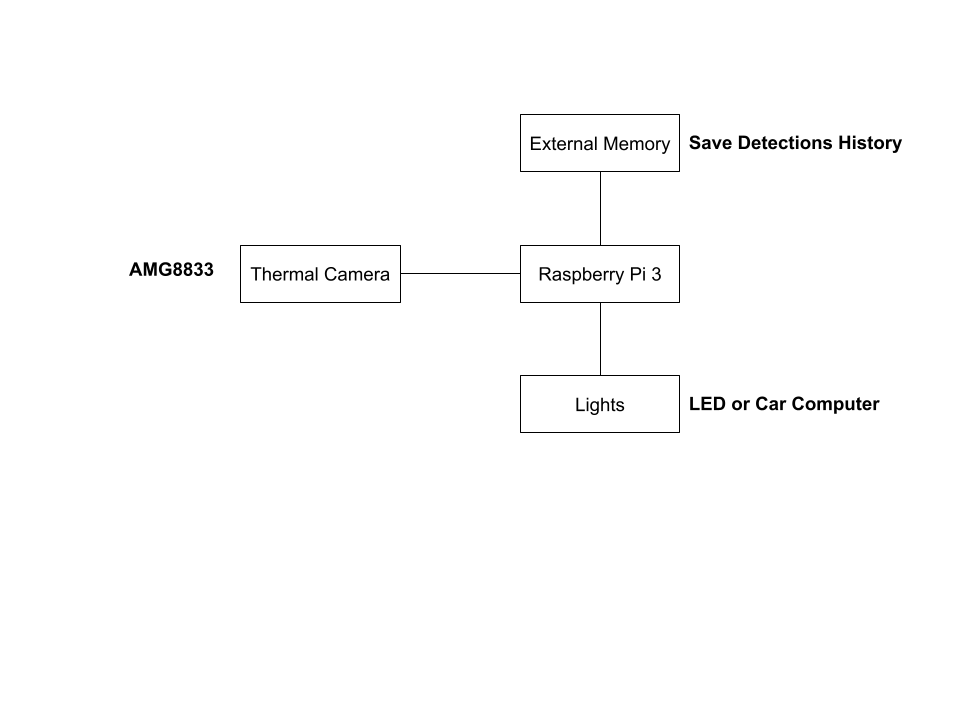
\includegraphics[scale=0.5]{figs/arch.png}

	\caption{معماری سطح بالای سیستم}
	\label{fig:1}
\end{figure}